\subsection{Mutation}
\label{subsec:Mutation}
Im Allgemeinen wird versucht mit Hilfe von Mutationsmechanismen aus einem
bestehenden Individuum, ein Individuum mit neuen Eigenschaften zu erzeugen.
Dies geschieht nach \cite{ErbenSkript} indem aus dem Genpool aller Individuen,
zufällig ein Gen ausgwählt wird, das über einen bestimmten Mutations-Algorithmus
verändert wird. Über Mutation wird oft versucht neue Lösungen zu erzeugen, welche
alleine durch die Regeln der Selektion und Rekombination oft nicht erreicht werden
könnten. So wird nach \cite{url:UniPaderborn} durch Mutation 'eine
frühzeitige Konvergenz eines Algorithmus verhindert'. Im Folgenden werden hierzu
die unterschiedlichen Mutationsoperatoren 'mutswap ', 'mutmove' und  'mutinvert'
genauer betrachtet.

\subsection{Mutationsoperator 'mutswap'}
\label{subsec:mutswap}
Die Mutationsart 'mutswap' ist ein einfacher Algortihmus, bei dem nach 
\cite{url:geatbx-documentation} 'eine zufällig ausgwählte Variable eines
Indivduums, mit einer anderen Variable des selben Individuums vertauscht
wird'. Unter einer Variablen ist ein bestimmtes Gen eines Chromosoms zu
verstehen. Die folgende Abbildung \ref{fig:MUTSWAP} veranschaulicht dies.
Hierbei werden die Positionen der Variabeln mit den Werten $7$ und $3$
vertauscht.

\begin{figure} 
  \centering
  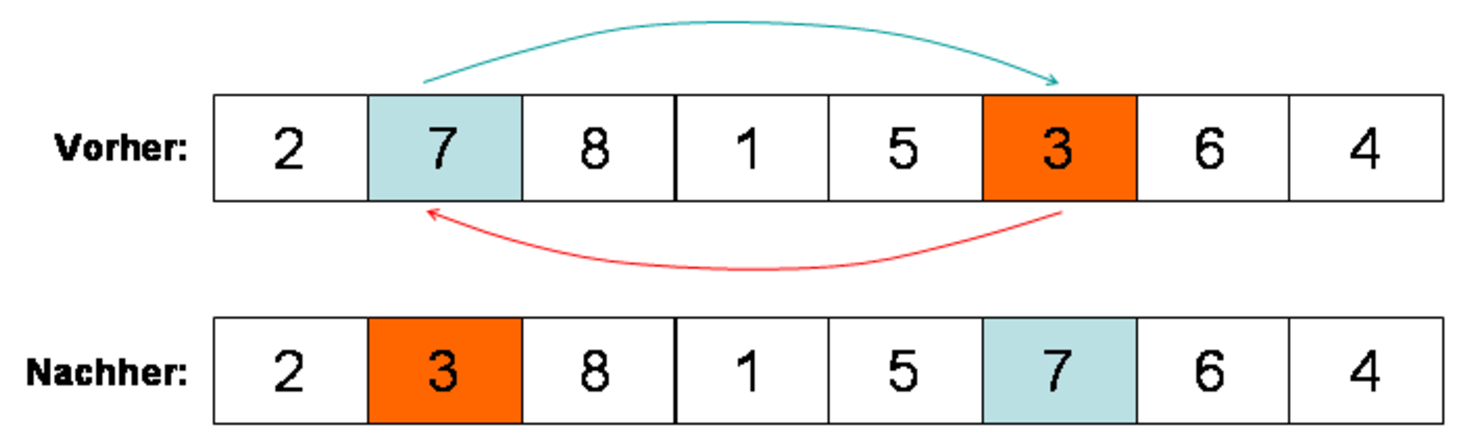
\includegraphics[width=0.7\textwidth]{../images/picMUTSWAP}
  \caption{Mutation mit 'mutswap'-Operator}
  \label{fig:MUTSWAP}
\end{figure}

\subsection{Mutationsoperator 'mutmove'}
\label{subsec:mutmove}
Bei der 'mutmove'-Methode handelt es sich um eine Mutation, bei der 
die Position \textit{i} einer Variabeln  innerhalb eines Chromosoms
an eine neue Position \textit{k} verschoben wird. Alle Variabeln
mit Positionen ab \textit{i+1} bis \textit{k} rutschen während
der Verschiebung um eine Position nach vorne.  
Abbildung \ref{fig:MUTMOVE} verdeutlicht dies. Hierbei wird
die Variable mit dem Wert $7$ um vier Positionen nach rechts verschoben.
Dabei rutschen die Variabeln mit den Werten $8$, $1$, $5$ und $3$ um je
eine Position nach vorne.

\begin{figure} 
  \centering
  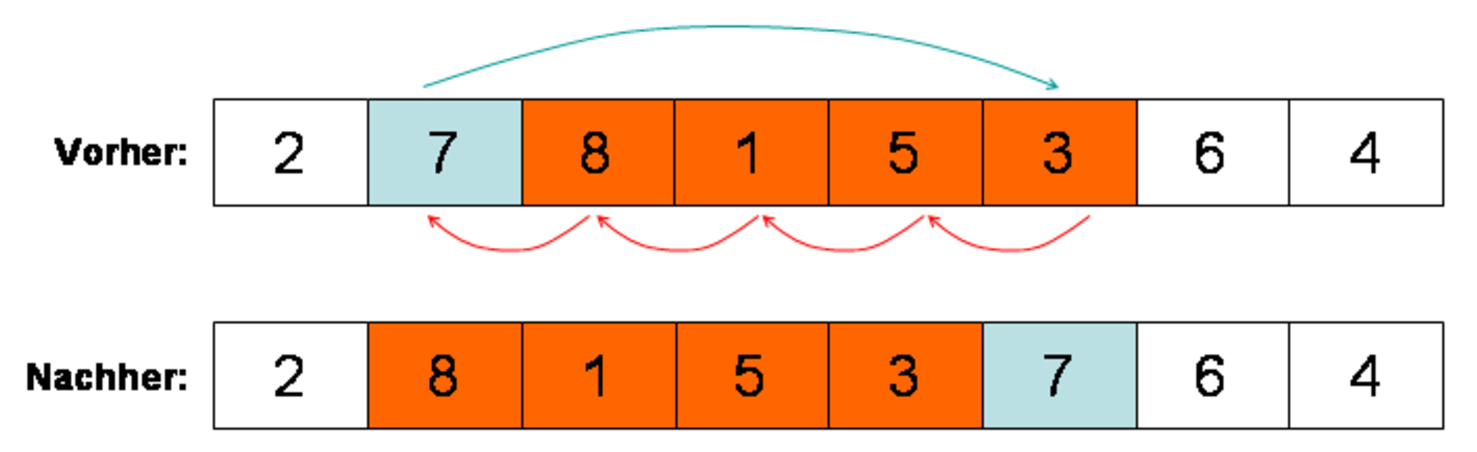
\includegraphics[width=0.7\textwidth]{../images/picMUTMOVE}
  \caption{Mutation mit 'mutmove'-Operator}
  \label{fig:MUTMOVE}
\end{figure}

\subsection{Mutationsoperator 'mutinvert'}
\label{subsec:mutinvert}
Bei Verwendung des 'mutinvert'-Operators wird nach
\cite{url:geatbx-documentation} 'jede Variablen-Position innerhalb
zweier Positionen invertiert'. D. h. es wird zuerst die Sequenz
oder Gruppe von Variabeln ermittelt, die zwischen zwei zufälligen
Positionen liegen. Die Positionen dieser Sequenz-Gruppe werden
anschließend invertiert. Abbildung \ref{fig:MUTINVERT} zeigt wie
aus der Sequenz $8$, $1$, $5$, $3$, die Sequenz $3$, $5$, $1$, $8$
entsteht.   

\begin{figure} 
  \centering
  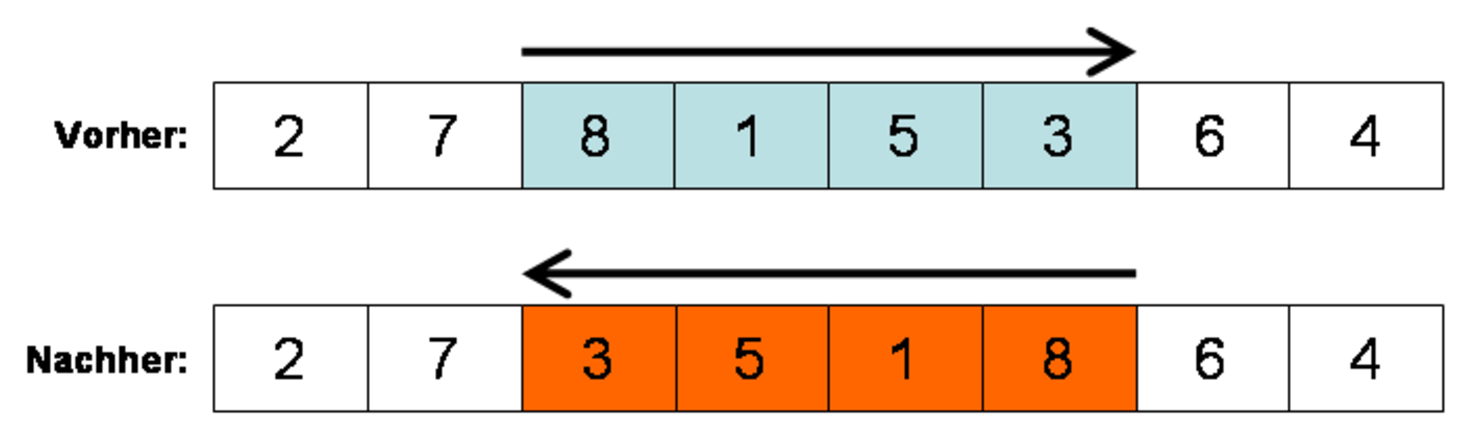
\includegraphics[width=0.7\textwidth]{../images/picMUTINVERT}
  \caption{Mutation mit 'mutinvert'-Operator}
  \label{fig:MUTINVERT}
\end{figure}

\subsection{Einsatz aller Mutationsoperatoren}
\label{subsec:AlleMutationen}
Wie am Anfang des Kapitels \ref{subsec:Mutation} beschrieben, ist das
Ziel bei der Mutation, neue Eigenschaften bei Individuen zu erzeugen.
Würde man nun 1 Mutationsart einsetzen, so könnte es vorkommen, dass
ein bereits ein oder mehrfach mutiertes Individuum, wieder in seinen
Ausgangszustand vor der ersten Mutation versetzt wird. Des Weiteren
könnte es vorkommen, dass eine bereits bestehende Veränderung im Erbgut der
Nackommen ebenfalls wieder zurückmutiert werden würde. D.h. man
würde durch erneutes Anwenden quasi alle Mutationsschritte rückgängig machen.
So wäre es möglich, dass bei 'mutswap' exakt die gleichen Variabeln
zurückgetauscht werden würden. Achtmaliges Anwenden der Operation 
'mutmove', würde eine Variable bspw. wieder an ihre
Ausgangsposition zurückversetzen. Auch bei 'mutinvert' wäre es möglich,
dass eine bereits invertierte Sequenz zurück invertiert wird.

Abbildung \ref{fig:MUTINVERTBackchange} illustriert am Beispiel von 'mutswap'
das unerwünschte Ergebnis nach mehrfachen Anwenden derselben Mutation.

Aus diesem Grund mischt man die angesprochenen Mutationsverfahren innerhalb
eines Testlaufs. Dadurch minimiert sich die Wahrscheinlichkeit, mit derselben
Mutationsart, eine bereits erreichte und gewünschte Veränderung des
Erbgutes wieder versehentlich rückgängig zu machen.
 
\begin{figure} 
  \centering
  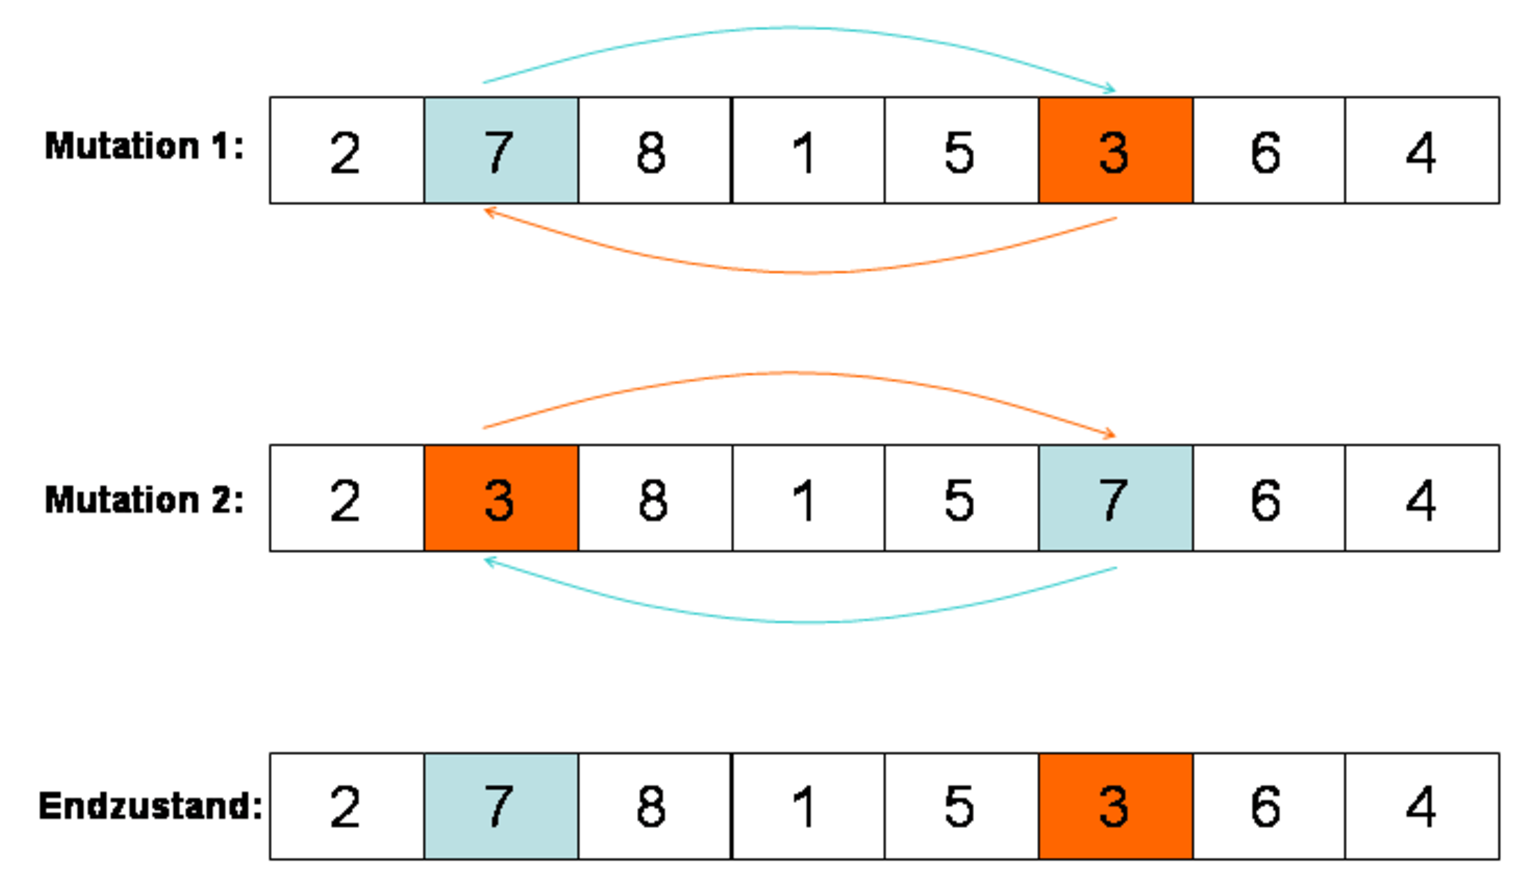
\includegraphics[width=0.6\textwidth]{../images/picMUTINVERTBackchange}
  \caption{Unerwünschter Zustand nach zweimaligen Anwenden von 'mutswap'.}
  \label{fig:MUTINVERTBackchange}
\end{figure}

\subsection{Testläufe mit variierenden Mutationsraten}
\label{subsec:TestlaufeMuationsraten}
Für die Durchführung der Testreihen in Aufgabe f), wurde eine 
angepasste Version des \ref{subsec:ArchitekturTestsystem} beschriebenen
Testskriptes benutzt.

\begin{description}
  \item[Mutations-Verfahren:] 'mutswap', 'mutmove', 'mutinvert' (kombiniert)
  \item[Mut.-Raten:] 0.001, 0.005, 0.01, 0.05, 0.08, 0.1, 0.2, 0.3, 0.4, 0.5, 1, 3, 5, 10, 15, 20, 25
\end{description} 

Es wurden 16 Testreihen, mit jeweils 20 Testläufen durchgeführt. Jeder der
Testläufe wurde mit einer Kombination der drei Muationsarten durchgeführt.
Zwischen den einzelnen Testläufen wurde die Muationsrate variiert.
Die Ergebnisse aller Testläufe werden hierzu in Tabelle
\ref{tbl:aufgabeF-ergebnisse} dargestellt.

\begin{table}
	\sffamily
	\centering
	\footnotesize
	\begin{tabularx}{\textwidth}{NXlllll}
		\toprule
		\multicolumn{1}{@{}N}{Mut.-Rate} &
		\multicolumn{1}{V{3.5em}@{}}{Subpop.} &
		\multicolumn{1}{V{3.5em}@{}}{Indiv.} &
		\multicolumn{1}{V{5em}@{}}{Mittelwert $\bar{x}$} &
		\multicolumn{1}{V{6.5em}@{}}{Standardabw. $\sigma_x$} &
		\multicolumn{1}{V{9em}@{}}{Minimalwert in Lauf $r$, Generation $g$} &
		\multicolumn{1}{V{9em}@{}}{Maximalwert in Lauf $r$, Generation $g$} \\
		\midrule\addlinespace
		
		0.001 & 12 & 60 & 2387.95 & 110.29 & 2217 , $r = 8$, $g = 100$ & 2611 , $r = 18$, $g = 92$ \\ \cmidrule(lr){1-7}
		0.005 & 12 & 60 & 2170.20 & 80.31 & 2062 , $r = 11$, $g = 97$ & 2422 , $r = 16$, $g = 94$ \\ \cmidrule(lr){1-7}
		0.01 & 12 & 60 & \textbf{2138.45} & \textbf{58.19} & 2059 , $r = 7$, $g = 87$ & \textbf{2249} , $r = 4$, $g = 99$ \\ \cmidrule(lr){1-7}
		0.05 & 12 & 60 & 2223.45 & 101.40 & 2084 , $r = 1$, $g = 97$ & 2423 , $r = 18$, $g = 94$ \\ \cmidrule(lr){1-7}
		0.08 & 12 & 60 & 2379.30 & 156.63 & 2121 , $r = 16$, $g = 96$ & 2633 , $r = 14$, $g = 88$ \\ \cmidrule(lr){1-7}
		0.1 & 12 & 60 & 2456.35 & 124.13 & 2257 , $r = 16$, $g = 95$ & 2742 , $r = 7$, $g = 83$ \\ \cmidrule(lr){1-7}
		0.2 & 12 & 60 & 2772.90 & 136.93 & 2613 , $r = 8$, $g = 99$ & 3072 , $r = 14$, $g = 74$ \\ \cmidrule(lr){1-7}
		0.3 & 12 & 60 & 3029.95 & 131.85 & 2834 , $r = 15$, $g = 84$ & 3372 , $r = 2$, $g = 72$ \\ \cmidrule(lr){1-7}
		0.4 & 12 & 60 & 2159.30 & 69.12 & 2047 , $r = 11$, $g = 100$ & 2278 , $r = 13$, $g = 100$ \\ \cmidrule(lr){1-7}
		0.5 & 12 & 60 & 2171.20 & 93.45 & \textbf{2026} , $r = 8$, $g = 92$ & 2339 , $r = 16$, $g = 93$ \\ \cmidrule(lr){1-7}		
		1 & 12 & 60 & 2217.30 & 89.41 & 2065 , $r = 3$, $g = 86$ & 2403 , $r = 2$, $g = 95$ \\ \cmidrule(lr){1-7}
		3 & 12 & 60 & 2449.45 & 110.05 & 2229 , $r = 13$, $g = 100$ & 2606 , $r = 2$, $g = 90$ \\ \cmidrule(lr){1-7}
 	 	5 & 12 & 60 & 2677.10 & 138.78 & 2424 , $r = 1$, $g = 93$ & 2898 , $r = 20$, $g = 72$ \\ \cmidrule(lr){1-7}
		10 & 12 & 60 & 3061.95 & 172.52 & 2769 , $r = 13$, $g = 92$ & 3334 , $r = 12$, $g = 90$ \\ \cmidrule(lr){1-7}
		15 & 12 & 60 & 3287.40 & 161.55 & 2997 , $r = 17$, $g = 100$ & 3582 , $r = 13$, $g = 95$ \\ \cmidrule(lr){1-7}
		20 & 12 & 60 & 3395.55 & 110.47 & 3151 , $r = 20$, $g = 53$ & 3600 , $r = 5$, $g = 95$ \\ 
								
		\addlinespace\bottomrule
		\end{tabularx}
	\caption{Ergebnisse aus 16 Testreihen a 20 Testläufe, mit kombinierten Mutationsverfahren und unterschiedlichen Mutationsraten.}
	\label{tbl:aufgabeF-ergebnisse}
\end{table}

\subsubsection{Interpretation der Ergebnisse}
Tendenziell zeigt sich durch eine Erhöhung der Mutationsrate eine eher negative
Auswirkung auf die einzelnen Testergebnisse. So führen die hohen Mutationsraten
ab '1', zu einer deutlichen Verschlechterung der Werte. Auch die Ergebnisse zwischen
den Raten '0.1' und '0.3', verschlechtern sich zusehens mit der Erhöhung.
Die besten Ergebnisse konnten mit Mutationsraten zwischen '0.005' bis '0.05',
sowie '0.4' bis '1' erzielt werden. Der minimalste Wert von 2026 Kilometern, 
wurde dabei mit der Mutationsrate von '0.5' erreicht. Das durschnittlich
beste Ergebnis wurde mit der Mutationsrate von '0.01' und einem Mittelwert von
2138.45 erzielt. Die Standardabweichung von 58.19, weist dabei ebenfalls den 
niedrigsten Wert aller Testläufe auf. 
